\documentclass[journal]{IEEEtran}

\usepackage{graphicx}
\usepackage{graphicx}
\graphicspath{{img/}}
\DeclareGraphicsExtensions{.pdf,.jpeg,.png}

% correct bad hyphenation here
\hyphenation{op-tical net-works semi-conduc-tor}

\usepackage[style= ieee, 
            urldate=comp,
            backend= biber]{biblatex}
\usepackage{xpatch}
\usepackage{url}

\begin{filecontents*}{\jobname.bib}
@misc{SPOF,
 title={Definition Single Point of Failure},
 url={https://en.wikipedia.org/wiki/Single_point_of_failure},
 note={(Date last accessed 11-August-2017)},
 }
 
@BOOK{Rastocny2013,
  author = {Rástočný, Karol and Ždánsky, Juraj},
  title = {Riadiace systémy so safety PLC},
  year = {2013},
  pages = {203},
  publisher = {VÚŽ Praha},
  owner = {Jaroslav Fait},
  timestamp = {2017.05.03},
  url = {http://librarian/stable.php?id=261}
}

\end{filecontents*}
\addbibresource{\jobname.bib}

\begin{document}
%
% paper title
\title{Design Power Supply with Uvervoltage Protection \\
       Acceptable for SIL4  application According EN50129}

\author{Jaroslav~Fait} 

% The paper headers
\markboth{WayGuard Project: RA\_HW002,~Vol.~1, No.~1, August~2017}%
{Shell \MakeLowercase{\textit{et al.}}: Bare Demo of IEEEtran.cls for IEEE Journals}

% make the title area
\maketitle

% As a general rule, do not put math, special symbols or citations
% in the abstract or keywords.
\begin{abstract}
  This abstract is aimed for Number specification.
\end{abstract}

% Note that keywords are not normally used for peerreview papers.
\begin{IEEEkeywords}
  SIL4, WayGuard, Bistabil relay
\end{IEEEkeywords}




% For peer review papers, you can put extra information on the cover
% page as needed:
% \ifCLASSOPTIONpeerreview
% \begin{center} \bfseries EDICS Category: 3-BBND \end{center}
% \fi
%
% For peerreview papers, this IEEEtran command inserts a page break and
% creates the second title. It will be ignored for other modes.
\IEEEpeerreviewmaketitle


\section{Single Points of Failure in a simple setup}
  Systems can be made robust by adding redundancy in all potential SPOFs (single point of failure) 
  \cite{SPOF}. For example on the figure \ref{HW002:fig006}, two sensors are powered by simplex 
  element - power source. If the power supply breaks (overvoltage/undervoltage), it can compromise 
  any safety margin gained in using dual sensors. 
  
  \begin{figure}[!ht] %\ref{HW002:fig006}
    \centering
    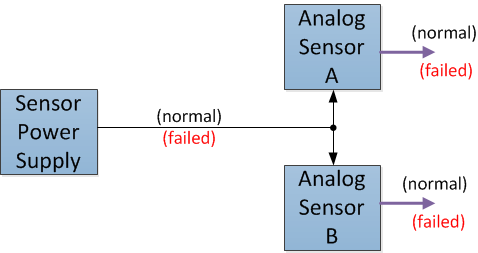
\includegraphics[width=0.6\linewidth]{fig_HW006.png}
    \caption{Simplex component failure may brings in matching but incorrect results in the dual 
             sensors}
    \label{HW002:fig006}
  \end{figure}
  
    Redundancy can be achieved at various levels. The assessment of a potential SPOF involves 
    identifying the critical components of a complex system that would provoke a total systems 
    failure in case of malfunction. Highly reliable systems should not rely on any such individual 
    component.

\section{Dual Computer Architecture}
  
  When microcomputers were introduced in mid 1980s, diagnostic functions became the main force of 
  the CPUs. In applying microcomputers to railway signalling, conventional safety measures based on 
  the asymmetric nature of component failure modes are not available. Instead, however, 
  microcomputers enable high-frequency diagnosis, and this leads to composite fail-safety and 
  reactive fail-safety as well \cite{Rastocny2013}. 
  
  The Dual Computer Architecture is the adoption of identical duplicate CPU configuration 
  (identical software).  Computer hardware, power supply, and interconnects (and
  sensors) are all duplicated, as is shown in figure \ref{HW002:fig005}. Each of the groups is 
  referred to as a channel.
  

  \begin{figure}[!ht] %\ref{HW002:fig005}
    \centering
    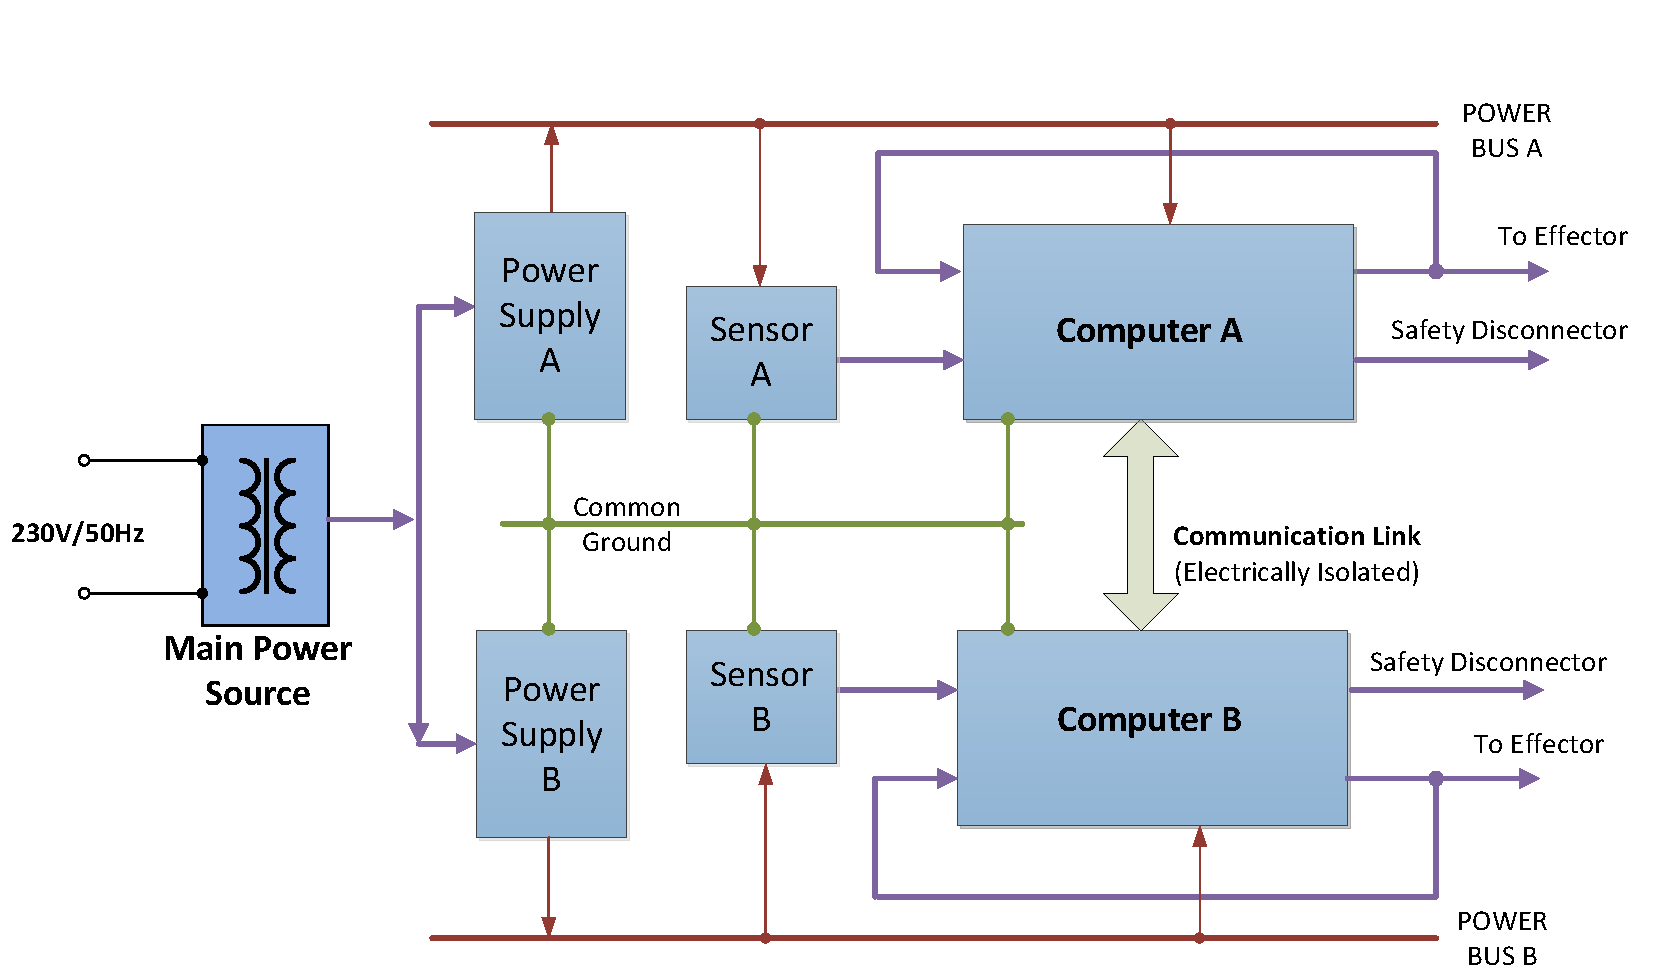
\includegraphics[width=1\linewidth]{fig_HW005.pdf}
    \caption{Redundant CPU Architecture }
    \label{HW002:fig005}
  \end{figure}

  Assumption:
  \begin{enumerate}
    \item Hardware in the channels is independent: A hardware failure in a channel has no effect 
          on the correct performance of other channels.
    \item The communication path is electrically isolated from the computers: A hardware failure 
          (such as a short circuit) in the connecting path will not propagate to computers.
   \end{enumerate}
   
  In safety discussion, whether or not a safe state can be defined also plays a big role power 
  supply concept, because wrong supplying can easy lead to \emph{common cause failure}.
  
  A common cause failure occurs when several failures have the same origin. Common cause failures 
  are either common event failures, where the cause is a single external event, or common mode 
  failures, where two systems fail in the same way for the same reason. Common mode failures can 
  occur at different times because of a design defect or a repeated external event
  
  For example overvoltage on the Main Power Supply's output on figure \ref{HW002:fig005} can leads 
  to same failure of all Auxiliary Power supplies, which can compromise all parts of the Fail-Safe. 
  
  The benefit of component duplication can be defeated by \emph{common-cause failure} (CCF) or 
  \emph{common-mode failures} (CMF)
  
\section{Crowbar Protection}
  \textbf{Crowbar protection} is a fail-safe protection mechanism which pulls the voltage below the 
  trigger level, usually close to ground. A clamp prevents the voltage from exceeding a preset 
  level. Thus, a crowbar will not automatically return to normal operation when the overvoltage 
  condition is removed; power must be removed entirely to stop its conduction. Crowbar protection 
  can also refer to a circuit which has its sole purpose to cause a fuse to blow by subjecting it 
  to high current.

  \begin{figure}[!ht] %\ref{HW002:fig003}
    \centering
    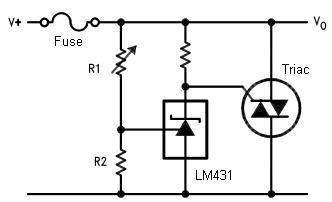
\includegraphics[width=0.6\linewidth]{fig_HW003.jpg}
    \caption{Simple Crowbar Protection with SCR}
    \label{HW002:fig003}
  \end{figure}

  \begin{figure}[!ht] %\ref{HW002:fig004}
    \centering
    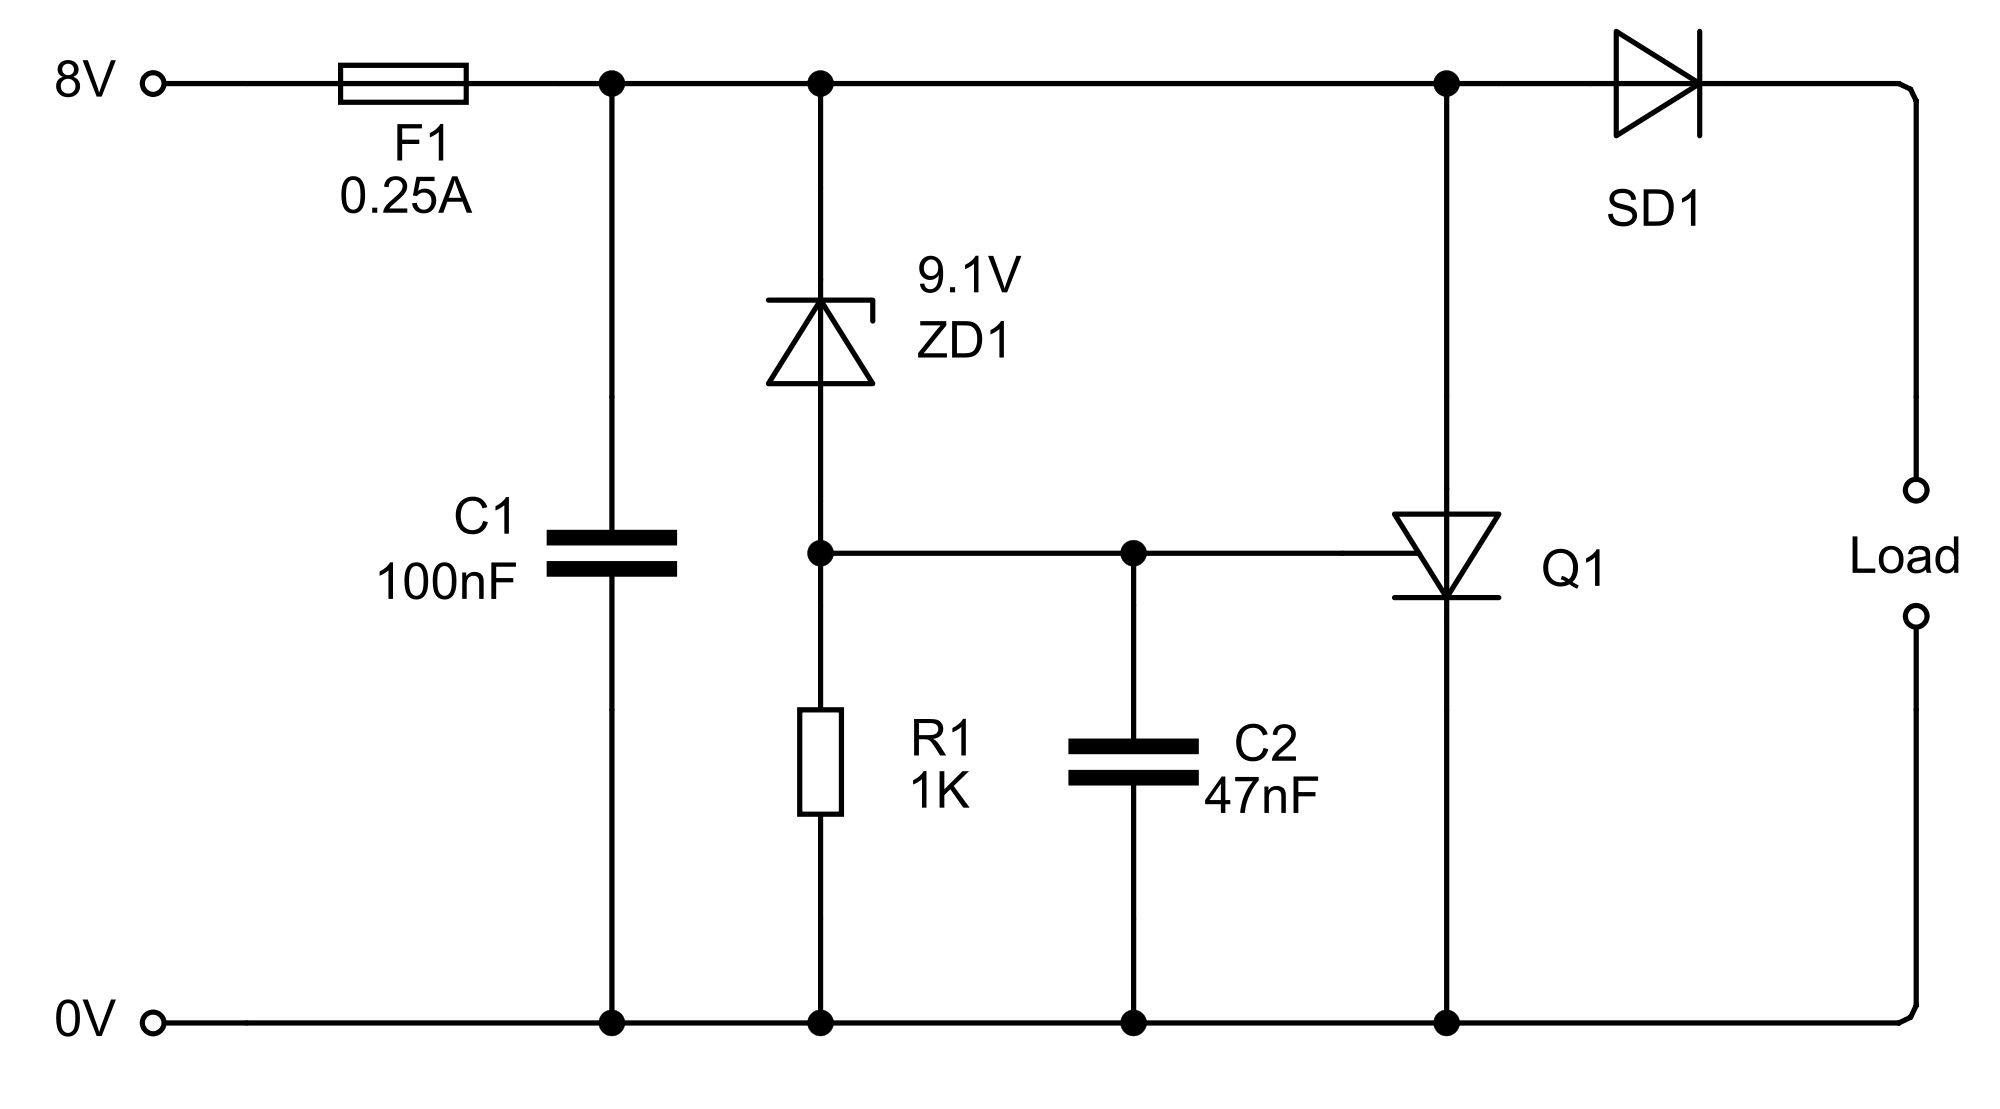
\includegraphics[width=0.6\linewidth]{fig_HW004.png}
    \caption{Simple Crowbar Protection with SCR}
    \label{HW002:fig004}
  \end{figure}
  
\nocite{*}
\printbibliography
\end{document}